%!TEX program=xelatex
\documentclass[a4paper]{article}
\usepackage{ctex}
\usepackage{geometry}
\usepackage{graphicx}
\usepackage{float}
\usepackage{listings}
\usepackage{xcolor}
\lstset{
    numbers=left, 
    numberstyle= \tiny, 
    keywordstyle= \color{ blue!70},
    commentstyle= \color{red!50!green!50!blue!50}, 
    frame=shadowbox,
    rulesepcolor= \color{ red!20!green!20!blue!20} ,
    escapeinside=``,
    framexleftmargin=2em
}

\geometry{left=3.0cm,right=3.0cm,top=3.5cm,bottom=3.5cm}

\title{计数器 预习报告}
\author{2017011341, 陈旭}
\date{2019 年 5 月}

\begin{document}

\maketitle

\section{实验内容}

    \begin{itemize}
        \item 实现四位十进制计数器,支持清零。(千位不超过 1)
        \item 计数到学号末尾四位时停止计数。
    \end{itemize}

\section{实验原理}

    \subsection{计数}
        可选的计数芯片有十进制计数芯片(74LS90)和四位二进制同步计数芯片(74LS161),由于 74LS161 支持保持,因此在个位上使用 74LS161,而 74LS90 原生支持十进制计数,因此十位、百位使用 74LS90。千位上只显示 0/1,因此 1 对应的两段数码管常亮,只要控制 0 对应的数码管剩下的部分即可,这一部分使用一个 D 触发器实现反相即可。

    \subsection{进位}
        进位只要利用最高位(二进制第四位)的变化即可,从 7 到 8 时该位会从低电平上升到高电平,从 9 到 0 时又会从高电平下降到低电平,因此只要以该位下降沿作为高位(十进制位)的计数触发周期即可。
        由于 74LS161 原生不支持十进制计数,因此需要在其计数至 10 时进行置零操作。我的做法是这样的:当计数达到 9 时对 74LS161 进行同步置零,这样就会在下一次进位时将数清零。

    \subsection{清零}
        D 触发器、74LS161、74LS90 均有异步清零的功能,用按钮控制其异步清零即可。

    \subsection{学号}
        将学好对应的二进制中 1 的位置相与,在正常计数的情况下,学号对应数值时最小使得其为 1 的数值,用其控制 74LS161 的保持,即可实现计数至学号停止。

\section{电路图}

\begin{figure}[H]
    \centering
    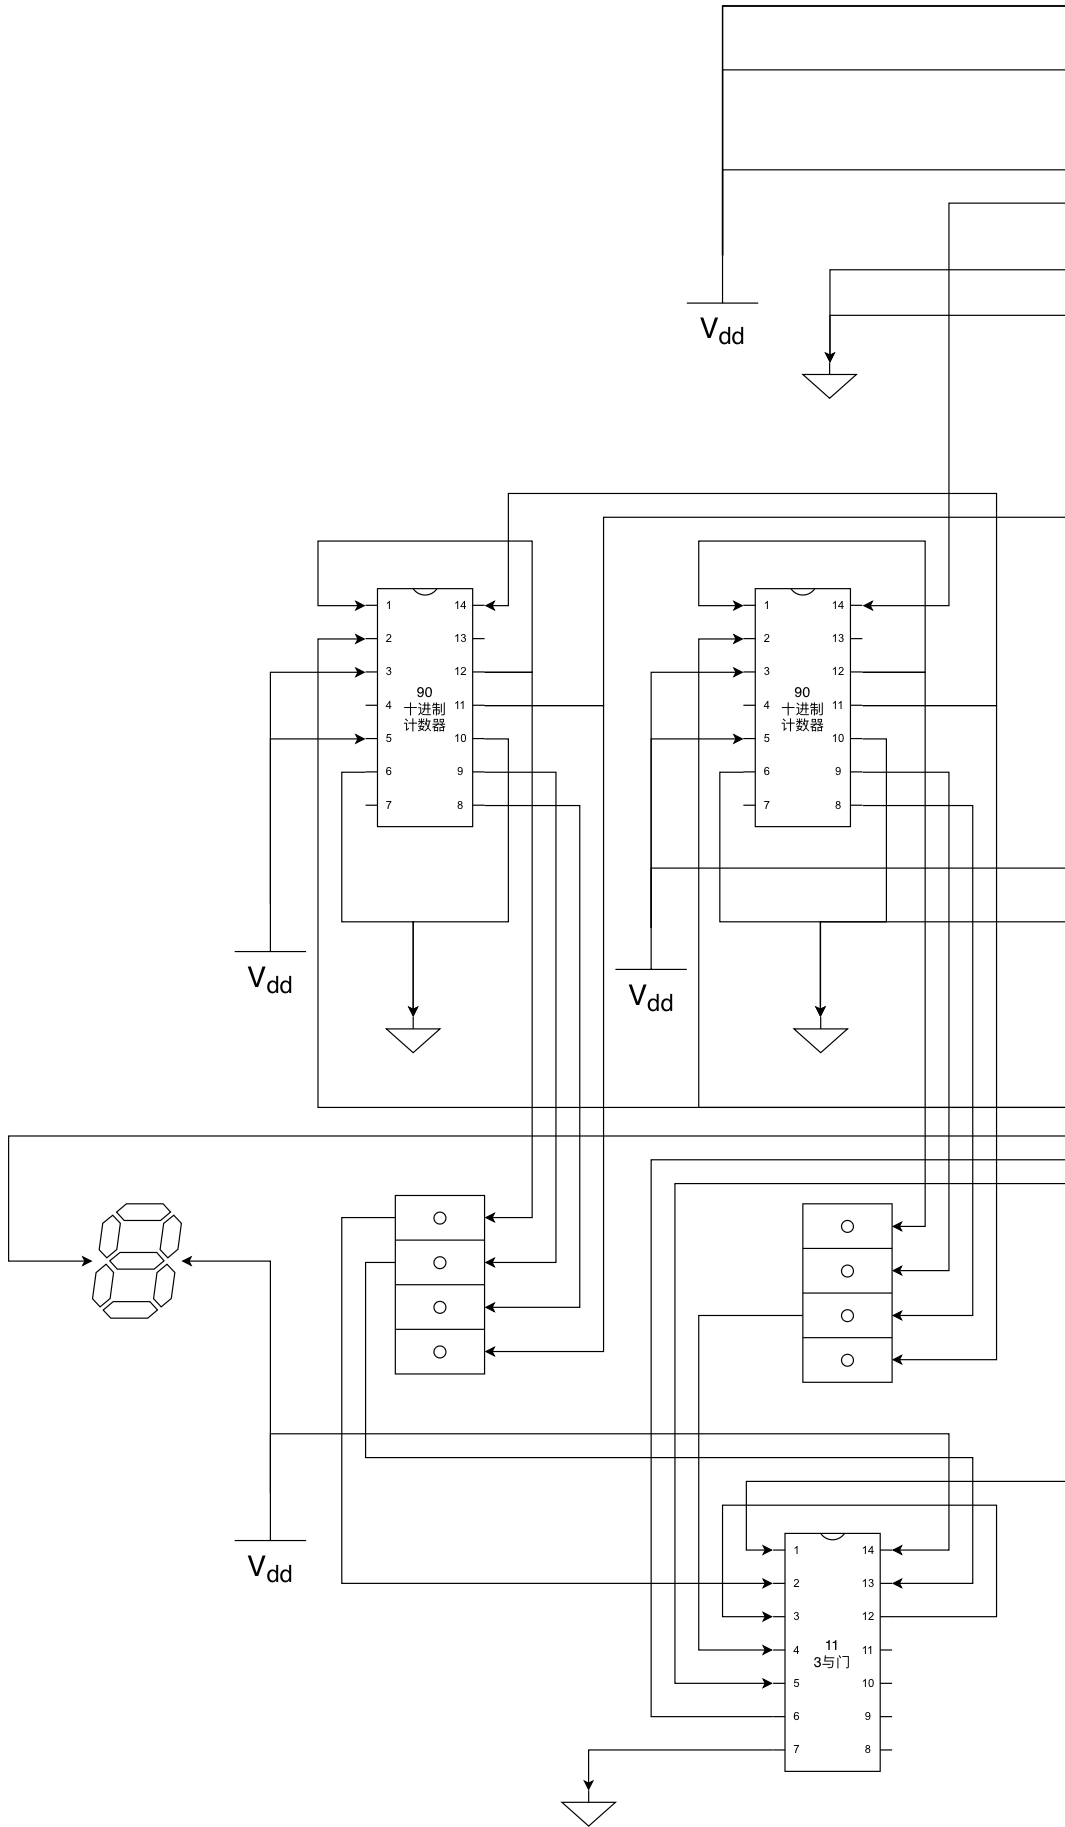
\includegraphics[width=0.8\linewidth]{figures/g1}
\end{figure}

\begin{figure}[H]
    \centering
    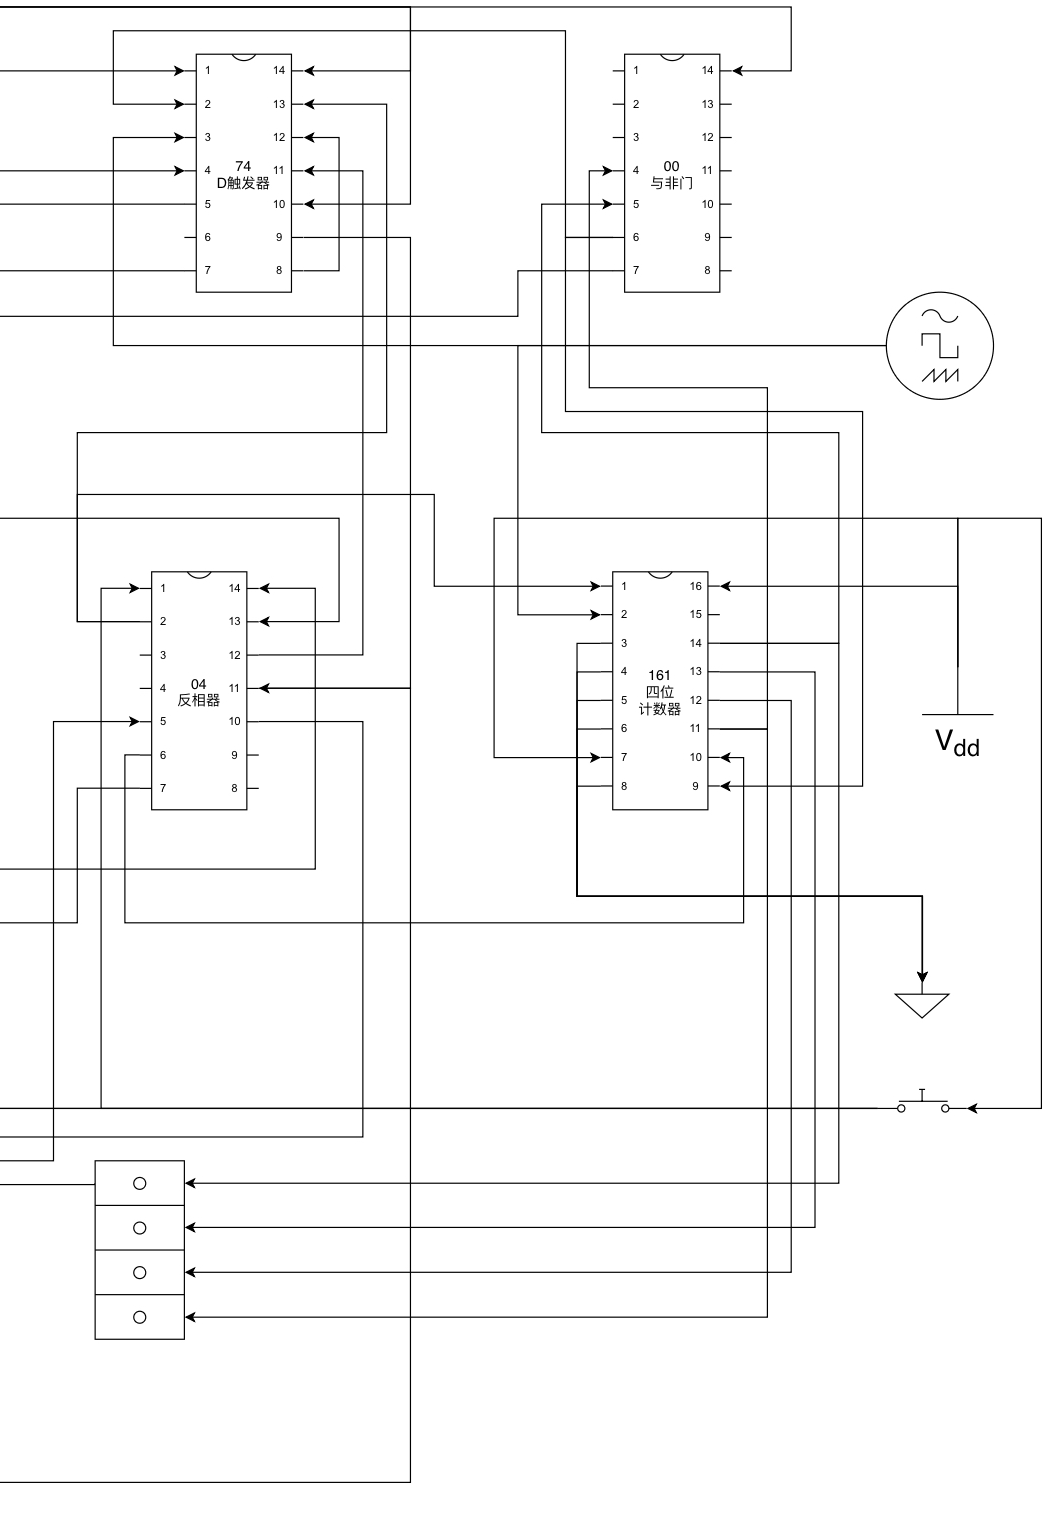
\includegraphics[width=0.9\linewidth]{figures/g2}
\end{figure}

\end{document}